\chapter{Design Architetturale}
\label{chap:architectural-design}
In questo capitolo verrà descritta l'architettura del sistema, illustrando i componenti principali. Si rimanda al capitolo \ref{chap:detailed-design} per ulteriori informazioni riguardante il codice dell'applicativo e le specifiche di implementazione.

\section{Architettura Generale}
L'architettura generale del sistema è illustrata nella figura \ref{pic:architecture}.

\begin{figure}[ht]
    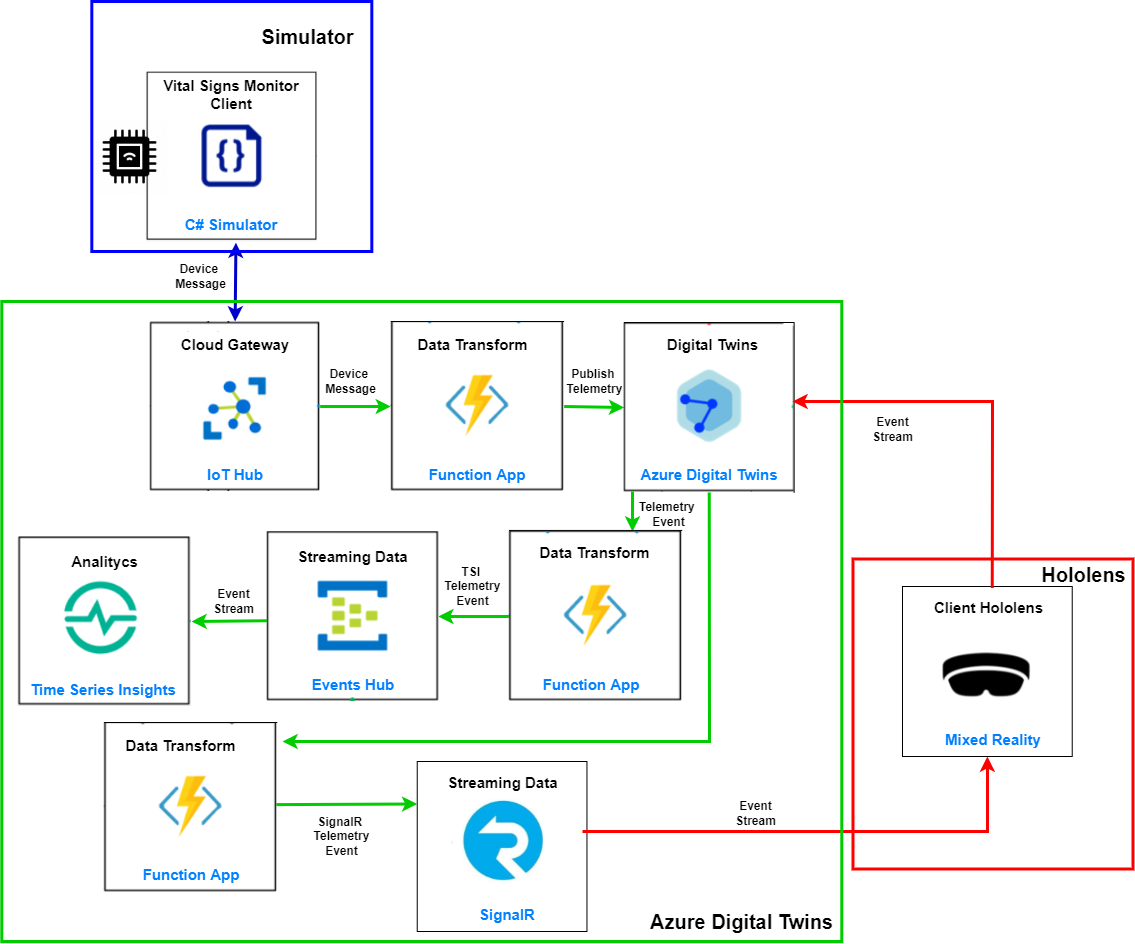
\includegraphics[width=10.3cm]{architecture.png}
    \centering
    \caption{\label{pic:architecture}Architettura del sistema.}
\end{figure}

Le componenti principali dell'architettura sono:

\begin{itemize}
    \item \textbf{Healthcare Vital Signs Monitor}: emula il monitor a parametri vitali fisico. Invia i dati ad Azure Digital Twins. Nella figura \ref{pic:architecture} è la componente blu;
    
    \item \textbf{Azure Digital Twins (ADT)}: una piattaforma PaaS fornita da Microsoft che mette a disposizione un'insieme di funzionalità per poter implementare e gestire i Digital Twins. Questa piattaforma permette di creare un gemello digitale dell'asset fisico, memorizzare un'insieme di dati che costituiscono lo stato del digital twin e propagarlo ad altri clients: in questo caso Hololens. Nella figura \ref{pic:architecture} è la componente verde;
    
    \item \textbf{Healthcare Hololens Client}: riceve lo stato dell'asset fisico da Azure Digital Twins tramite la libreria SignalR. Invia i dati di configurazione dell'ologramma ad Azure Digital Twins. Nella figura \ref{pic:architecture} è la componente rossa;  
\end{itemize}

\section{Healthcare Vital Signs Monitor}
Questa componente permette di creare la cartella clinica di un paziente compilando uno specifico form. Una volta completata viene creato il dispositivo IoT nell'IoT Hub e vengono creati i due digital twins in ADT: quello relativo al paziente e quello relativo al monitor a parametri vitali. A questo punto si è in grado eseguire il simulatore su uno specifico paziente. I parametri vitali monitorati dal simulatore sono cinque:

\begin{itemize}
    \item Temperatura corporea (colore bianco) misurata in gradi Celcius (°C);
    \item Frequenza cardiaca (colore verde) misurata in BPM (Beat per minute);
    \item Frequenza respiratoria (colore verde) misurata in RPM (Revolution per minute);
    \item Saturazione (colore rosso) misurata in percentuale (\%);
    \item Pressione sanguigna (di colore gialla) misurata in millimetri di mercurio o Torr (mmHg).
\end{itemize}

\begin{figure}[ht]
    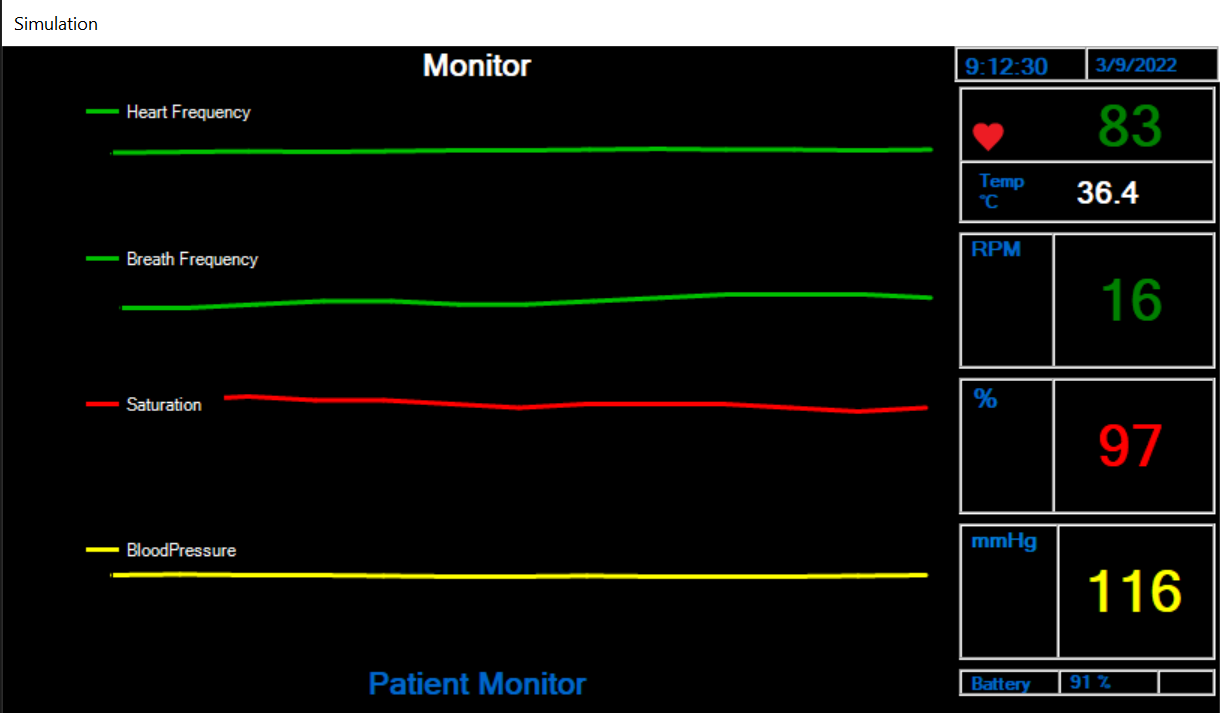
\includegraphics[width=11cm]{simulator.png}
    \centering
    \caption{\label{pic:simulator}Simulatore.}
\end{figure}

Come si evince dalla figura \ref{pic:simulator}, per tutti questi parametri vitali (eccetto la temperatura), è mostrato un grafico degli ultimi N campioni acquisiti con il colore di riferimento. \newline \newline Per tutti i parametri è presente anche un sensore di allerta (sia visivo che acustico) che si attiva se un valore supera (o diventa inferiore) il valore massimo (o minimo) di un determinato range (specifico per ogni parametro vitale). Tali sensori sono posti a sinistra dei grafici e alla destra del valore della temperatura e della batteria. Se si prende in considerazione l'immagine \ref{pic:simulator}, questi non sono visibili poiché tutti i valori sono nella norma. L'infermiere o il chirurgo possono personalizzare i range e l'unità di misura. \newline \newline A destra del simulatore invece possiamo individuare due colonne: la prima indica l'unità di misura usata per rappresentare il valore del parametro vitale mentre la seconda mostra il suo valore numerico. In alto a destra si trova la data e l'orario corrente mentre in basso a destra il livello della batteria rimanente.
\newline \newline Una volta che il simulatore è in esecuzione, ogni volta che ha nuovi dati, questi vengono trasmessi al ADT.

\section{Azure Digital Twins}
Questa è la componente più corposa del sistema che funge da server. I diversi componenti vengono descritti a seconda dell'ordine di esecuzione in accordo con l'immagine \ref{pic:architecture}:

\begin{itemize}

    \item \textbf{IoT Hub}: è l'Hub di Azure che offre un back-end per ospitare sul cloud e connettere qualsiasi dispositivo IoT. All'interno dell'Hub sono presenti i dispositivi IoT ``\textit{virtuali}" relativi a monitors a parametri vitali di specifici pazienti. Tali dispositivi vengono aggiunti nell'Hub quando viene compilata la cartella clinica di un nuovo paziente. Tali dispositivi ricevono i dati dal simulatore e li propagano all'istanza \textit{Azure Digital Twins} attraverso l'esecuzione di una \textit{azure function};
    
    \item \textbf{Azure function}: è un servizio cloud che fornisce l'infrastruttura e le risorse necessarie per eseguire le applicazioni. L'azure function in questione è chiamata \textit{ProcessHubToDTEvents}. Tale funzione è in grado di eseguire il parsing del contenuto del messaggio inviato dal simulatore e aggiornare le proprietà dei digital twins.
    
    \item \textbf{Azure Digital Twins}: rappresenta l'istanza dove risiedono i digital twins. Per ogni paziente creato esistono due digital twins: quello del paziente e quello del monitor a parametri vitali. Essi sono legati da una relazione ``\textit{un paziente ha un monitor associato}". Tramite questa istanza è possibile consultare lo stato delle proprietà dei digital twins e fare queries. Ogni qualvolta che i digital twins vengono aggiornati vengono eseguite in parallelo due azure function descritte nel punto successivo;
    
    \item \textbf{Azure functions}. La prima azure function è chiamata \textit{ProcessDTUpdatetoTSI} ed è dedicata a propagare lo stato dei digital twins al Time Series Insights (TSI). La seconda azure function è chiamata \textit{SignalRFunction} ed implementa la libreria SignalR per poter comunicare con il client Hololens. Tale funzione ha due sotto-funzioni: la prima (\textit{negotiate}) permette di creare la connessione con il client, la seconda (\textit{broadcast}) permette di inviare i dati al client;
    
    \item \textbf{Time Series Insights (TSI)}: è una soluzione per archiviare, visualizzare ed eseguire queries su grandi quantità di dati relativi a quelli generati dai dispositivi IoT. Nel nostro applicativo i dati vengono solamente archiviati. Una funzionalità futura potrebbe essere quella di eseguire delle queries a partire dai clients per mostrare uno storico dei dati prodotti dal simulatore;
    
    \item \textbf{SignalR}: SignalR è una libreria sviluppata da Microsoft che permette al server di inviare notifiche asincrone alle applicazioni clients creando una connessione bi-direzionale. Risulta essere performante per applicazioni \textit{real-time} come nel nostro caso.
\end{itemize}

\section{Healthcare Hololens Client}
L'ultima componente del nostro sistema è il client Hololens che permette di usare la mixed reality. Dopo aver indossato gli occhiali e avviata l'applicazione, è necessario scansionare il QR code del paziente. Quando il QR code viene riconosciuto viene mostrato l'ologramma del monitor a parametri vitali e la cartella clinica del paziente. Una volta avviato il simulatore, l'ologramma del monitor si popolerà di nuovi dati e aggiornerà i valori dei parametri. Per avere un maggior controllo sulla visualizzazione dei dati abbiamo pensato ad un menù interattivo con cui scegliere quale tipo di dato osservare: se visualizzare la situazione generale del paziente o focalizzarsi su un singolo parametro vitale. Grazie alla mixed reality, il grande vantaggio è dato dall'interazione dell'uomo con l'ologramma. Infatti è possibile spostare il monitor ovunque si voglia nello spazio reale, ``\textit{prendendolo}" appunto con le mani. Invece per cambiare schermata è possibile premere su uno dei pulsanti del menù interattivo. Per una maggiore comodità abbiamo pensato fosse utile far si che gli ologrammi si spostino automaticamente in base a dove l'uomo si sta muovendo o guardando nell'ambiente (ad esempio come la funzionalità \textit{follow me}). Per fare ciò, è possibile attivare il pulsante PIN \emoji{pushpin} premendolo (in alto a destra di ogni ologramma). Come impostazione predefinita, tale pulsante è disattivato: in questo modo gli ologrammi rimangono fermi nell'ambiente se non vengono spostati direttamente dall'uomo.

\subsection{QR Code}
La parte relativa alla lettura del QR Code non ha nessuna interfaccia di interesse. Una volta avviata l'app su Hololens verrà mostrato un \textit{loading progress} in attesa della lettura di un QR Code. Dopo aver mostrato il QR Code, se è valido, verrà mostrato il menù, il monitor a parametri vitali e la scheda del paziente. \newline \newline Per l'implementazione di questa parte ci siamo avvalsi del seguente \href{https://github.com/LocalJoost/QRCodeService}{\textit{repository}}.

\subsection{Menù Interattivo}
Il menù si presenta come nell'immagine \ref{pic:menu-hololens}. E' composto da sette pulsanti:
\begin{itemize}
    \item il pulsante \textit{Home} permette di visualizzare il monitor a parametri vitali di un paziente come quello mostrato nel simulatore;
    
    \item ogni pulsante, in riferimento ad un parametro vitale, permette di visualizzare il suo pannello dedicato;
    
    \item il pulsante \textit{Values} permette di visualizzare solamente i valori dei parametri vitali del paziente, senza mostrare grafici;
    
    \item il pulsante \textit{Exit} permette di uscire dal programma.
\end{itemize}

\begin{figure}[ht]
    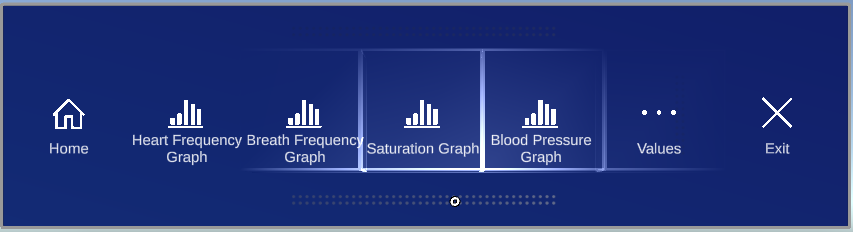
\includegraphics[width=11cm]{hololensMenu.PNG}
    \centering
    \caption{\label{pic:menu-hololens}Menu di Hololens.}
\end{figure}

\subsection{Monitor a parametri vitali}
L'immagine \ref{pic:example-hololens} mostra alcuni esempi: nella figura \ref{pic:monitor-hololens} è mostrato il monitor a parametri vitali generale mentre  nell'immagine \ref{pic:saturation-hololens} è presente il pannello dedicato ad un singolo parametro vitale. In questo caso si è scelto la saturazione premendo il pulsante \textit{Saturation Graph} dal menù. Durante la realizzazione dei pannelli della mixed reality si è cercato di preservare il più possibile la grafica del simulatore così da evitare confusione tra i due monitors: quello fisico e quello virtuale. \newline \newline Come descritto in precedenza, l'immagine \ref{pic:monitor-hololens} mostra a sinistra i sensori di allerta dei parametri vitali: di colore bianco quando i valori sono nella norma e di colore rosso quando assumono valori di pericolo per il paziente. Nell'esempio, la temperatura e la frequenza cardiaca sono in una situazione critica e vengono caratterizzati da un sensore di allarme di colore rosso. Proseguendo verso destra sono presenti i grafici dei quattro parametri vitali più importanti.
\begin{figure}
     \centering
     \begin{subfigure}[b]{0.8\textwidth}
         \centering
         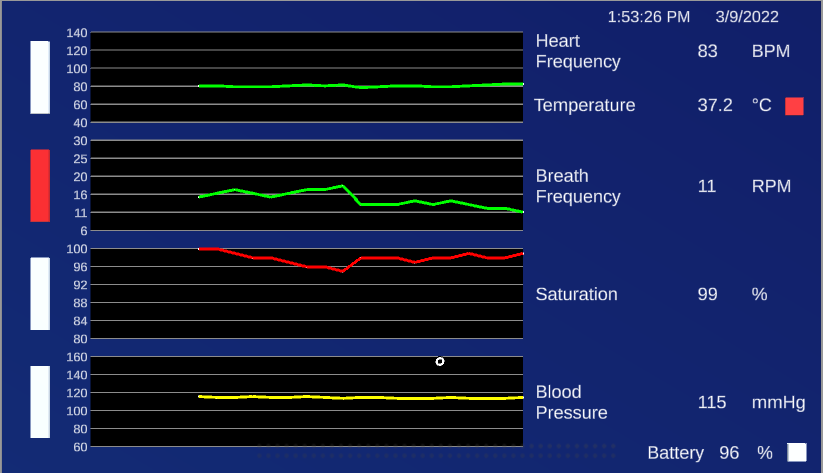
\includegraphics[width=\textwidth]{hololensMonitor.PNG}
         \caption{Monitor a parametri vitali generale.}
         \label{pic:monitor-hololens}
     \end{subfigure}
     \hfill
     \begin{subfigure}[b]{0.8\textwidth}
         \centering
         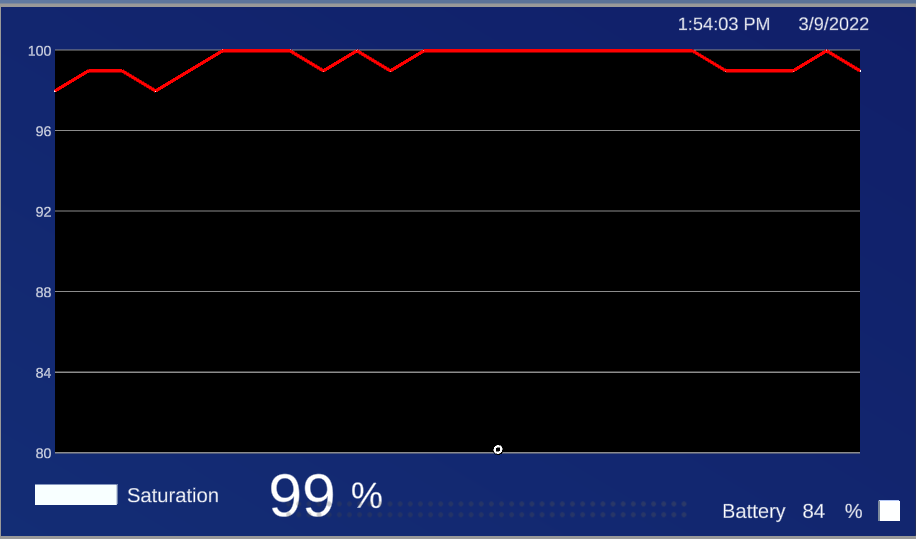
\includegraphics[width=\textwidth]{SaturationHololens.PNG}
         \caption{Monitor della saturazione.}
         \label{pic:saturation-hololens}
     \end{subfigure}
     \hfill
        \caption{Esempi di monitor a parametri vitali in Hololens.}
        \label{pic:example-hololens}
\end{figure}
Successivamente sono presenti tre colonne e contengono rispettivamente il nome del parametro vitale, il valore numerico e l'unità di misura utilizzata. \newline \newline La figura \ref{pic:saturation-hololens} mostra il pannello focalizzandosi su uno specifico parametro vitale. In questo modo si può osservare con più accuratezza e livello di dettaglio l'andamento del grafico. Tutti gli altri valori sono mostrati sotto il grafico.

\subsection{Pannello del Paziente}
L'ultimo ologramma è quello legato al paziente e mostra la sua cartella clinica. Tale pannello contiene le seguenti informazioni:
\begin{itemize}
    \item il nome e il cognome;
    \item il sesso;
    \item l'età, il peso e l'altezza
    \item l'indice di massa corporea;
    \item una descrizione riguardante la sua situazione clinica prima di entrare in sala operatoria. Può contenere note del team, il suo stato di salute e tutto ciò che è rilevante e da tenere in considerazione quando si effettua l'operazione;
    \item il suo codice fiscale;
\end{itemize}

Questo pannello contiene informazioni statiche poiché durante l'intervento queste non possono essere modificate. Il pannello del paziente si presenta come è mostrato nella figura \ref{pic:patient-panel}.

\begin{figure}[ht]
    \includegraphics[width=9.5cm]{PatientPanel.PNG}
    \centering
    \caption{\label{pic:patient-panel}Esempio del pannello del paziente.}
\end{figure}